%
% Appendix 2
%

\chapter{Boosted Decision Trees}
\label{app:bdts}


\section{Technical Description}

Boosted Decision Trees are the single MVA/machine learning technique used for discriminating signal from background
in this analysis. BDTs are used in this analysis exclusively for classification.
BDTs are a special instance of a decision tree, which is illustrated below in Figure~\ref{fig:dec_tree}.
This analysis uses the BDT implementation in the Toolkit for Multivariate Analysis (TMVA) software~\cite{tmva}, based on the
C4.5 algorithm~\cite{C4.5}.
The choice of BDTs over other MVA methods such as artificial neural networks (aNNs) or support vector machines (SVMs) is motivated
by several factors. While the cut-based classification technique the BDT relies on is a theoretically less powerful classifier compared
to other more sophisticated MVAs such as aNNs, it typically offers the best ``out-of-the-box'' performance, requiring the least amount
of optimization to acheive near-maximum performance. This simiplicity also translates to faster training and evaluation times.
Additionally, BDTs are often more robust against over-training\footnote{Over-training, or ``over-fitting'' describes the loss of generalization (as well as performance)
between the training and testing/evaluation samples. Over-training occurs when the MVA learns statistical features of the training sets that are not present in
the testing/evaluation set.}. This practically translates to using more input variables, and/or smaller training samples than more sophisticated MVAs.
The conceptual description of BDT training is described in the following sections. 
 
\begin{figure}[hbtp]
 \begin{center}
   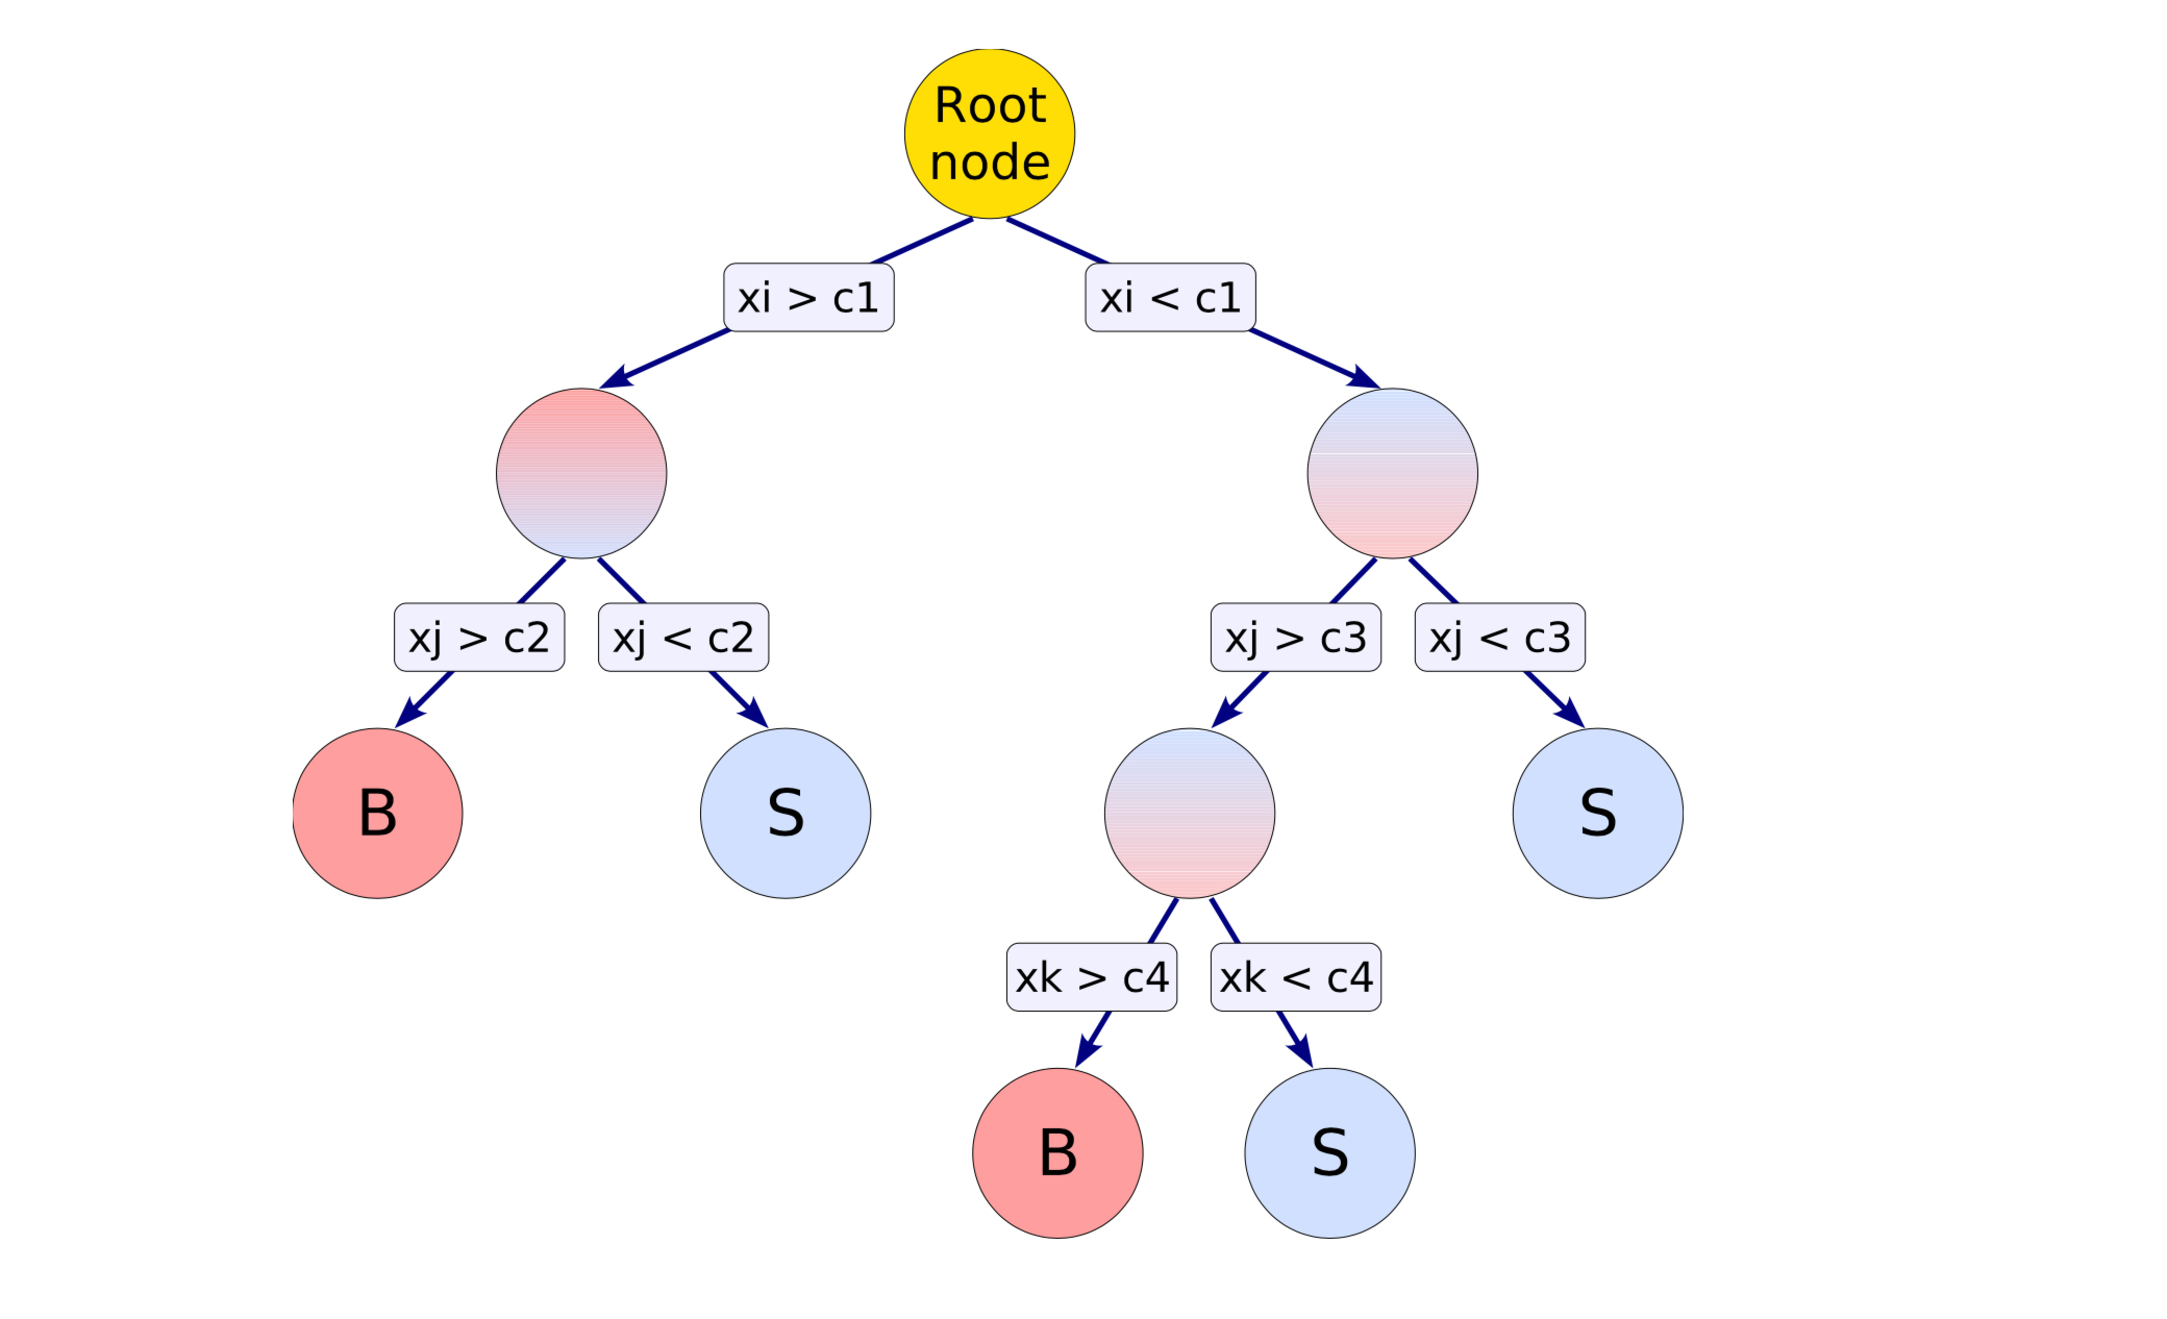
\includegraphics[width=0.8\textwidth]{ap2_figs/decision_tree.pdf}
   \caption[A decision tree diagram.]{An overview diagram of a single decision tree. The decision nodes are a mixture of red and blue,
     while the terminal nodes or leaves, are ideally depicted colored red or blue and labeled S or B for signal or background respectively~\cite{tmva}.}
   \label{fig:dec_tree}
 \end{center}
\end{figure}

\subsection{Tree Growth}
The decision tree begins at the root node with a single decision, or split. Given a set of inputs {$x$}, the input $x_{i}$, and the specific cut value $c_{1}$,
is selected based on best separation power between signal and background. The training events are then filtered through this first split, where events
with $x_{i} > c_{1}$ moving to the left forming a new decision node, and events with $x_{i} < c_{1}$ moving to the right, forming a new and separate 
decision node, as seen in Figure~\ref{dec_tree}. This processes is then repeated on the subsets of events in each of the two new nodes, and continued until
a specified stopping criteria is satisfied. This stopping criteria is often defined to be when a given split produces a node with purely signal or purely
background events, as illustrated in Figure~\ref{fig:dec_tree}. The stopping criteria consists of:
\begin{itemize}
\item Perfect classication
\item Not satisfying a specified minimum number of events (or fraction) of the training sample in the leaf
\item Insufficient improvement for available splittings
\item Reaching a specified maximum tree depth
\end{itemize}

One important detail not mentioned thus far is the metric used to determine ``best'' separation power when determining which variable and corresponding value to split on.
The first variable to consider for splitting criteria is purity of each node, defined as $p_{s}=\frac{s}{s+b}$, where $s$ and $b$ correspond to the number of signal and background
events in the node respectively. $p_{s}$ is 1 for a node with pure signal, and zero for a node with pure background. A $p{s}$ of 0.5 corresponds to equal amounts of signal and background
in the node. With a definition of purity, we define a figure of merit (FOM) called \textit{impurity}. The impurity of a given node $t$, is based on the purity and is denoted as
$\phi(t)$.
The impurity of a given node is maximized when the two classes (signal, background) are mixed in equal proportion $\phi(t) = 1/2$. The impurity is minimized when the node is pure
signal or pure background where $\phi(t) = 0$.
It makes more sense to work with the weighted impurities however, where a given node impurity is weighted by the number of events in that node. This quantity
will be referred to as weighted impurity $I(t) = \phi(t)N_{t}$, where $N_{t}$ is the number of events in the node. 
The splitting criteron maximizes the impurity gain, $\DeltaI(t)$. For a given node $t_{0}$ with $N_{0}$ events, we want to
select the best variable and value to split into two child nodes, $t_{L}$, with $N_{L}$ events, and $t_{R}$,with $N_{R}$ events, where $N_{0} = N_{L} + N_{R}$. Here, the
impurity gain for a given split is $\DeltaI(t) = I(t_{0}) - I(t_{L} - I(t_{R}))$, and we choose the cut which maximizes $\DeltaI(t)$ over all possible splits for all variables.
The functional form of $\phi(t)$ has not been given since there are a number of options. The simplest form of $\phi$ is the training error $\epsilon(t) = min(p_{s},p_{b})$.
The training error as the basis for the FOM suffers fro. To illustrate this shortcoming, see Figure~\ref{fig:tree_split}.

\begin{figure}[hbtp]
 \begin{center}
   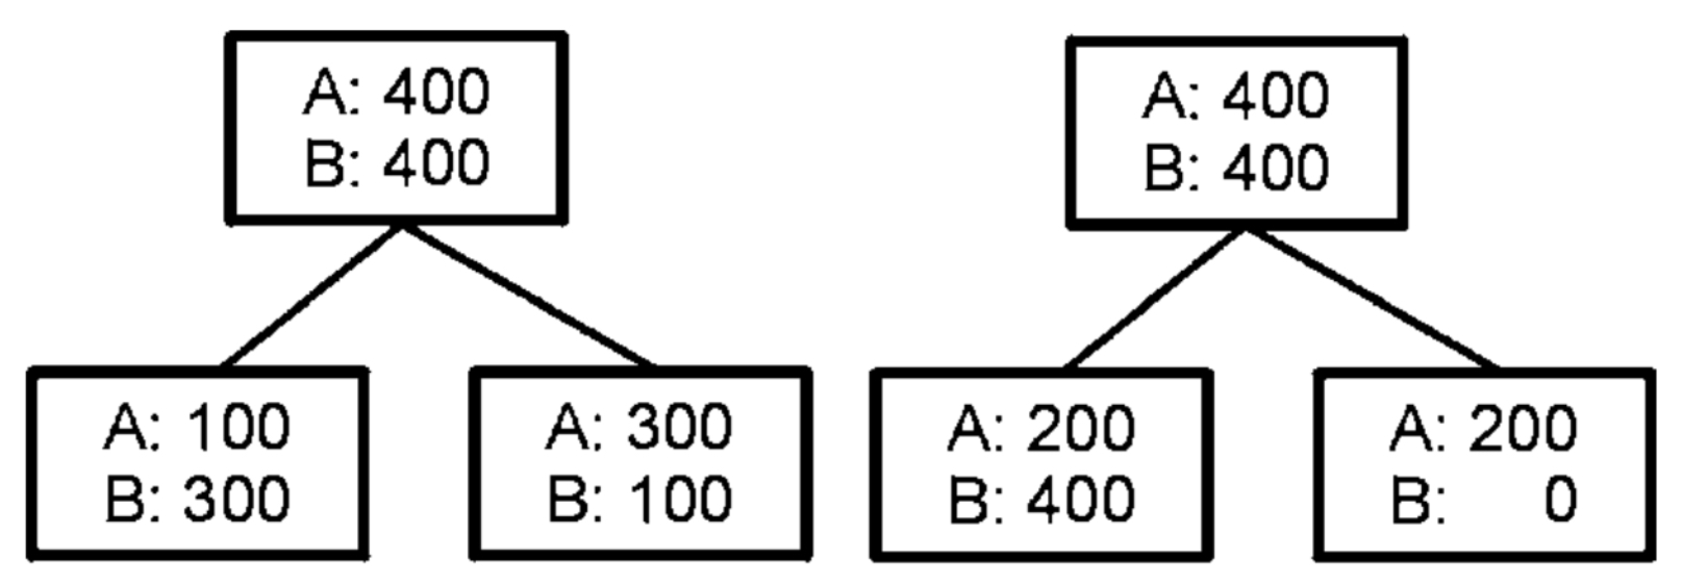
\includegraphics[width=0.5\textwidth]{ap2_figs/tree_split.pdf}
   \caption[Two splits with the same error rate.]{Two different splits that result in the same mis-classification error~\cite{illya}.}
   \label{fig:tree_split}
 \end{center}
\end{figure}

\noindent Both splits in Figure~\ref{fig:trees_plit} produce
the same training error (25$\%$), however the split on the right is clearly a more powerful separator. Other forms of $\phi$ that avoid this scenario by punishing
event mis-classifications non-linearly include the Gini index $\phi = 1 - p_{s}^{2} - p_{b}^{2}$, and the cross entropy $\phi = \frac{-p_{s}log(p_{s})+p_{b}log(p_{b})}{2}$.
The FOM used for the BDTs in this analysis is the Gini index, which punishes mis-classifications less severely for more equal distributions of signal and background, and more
severely for mis-classifications of very unequal distributions of signal and background in a node. This is demonstrated in Figure~\ref{fig:misclass_plot}.

\begin{figure}[hbtp]
 \begin{center}
   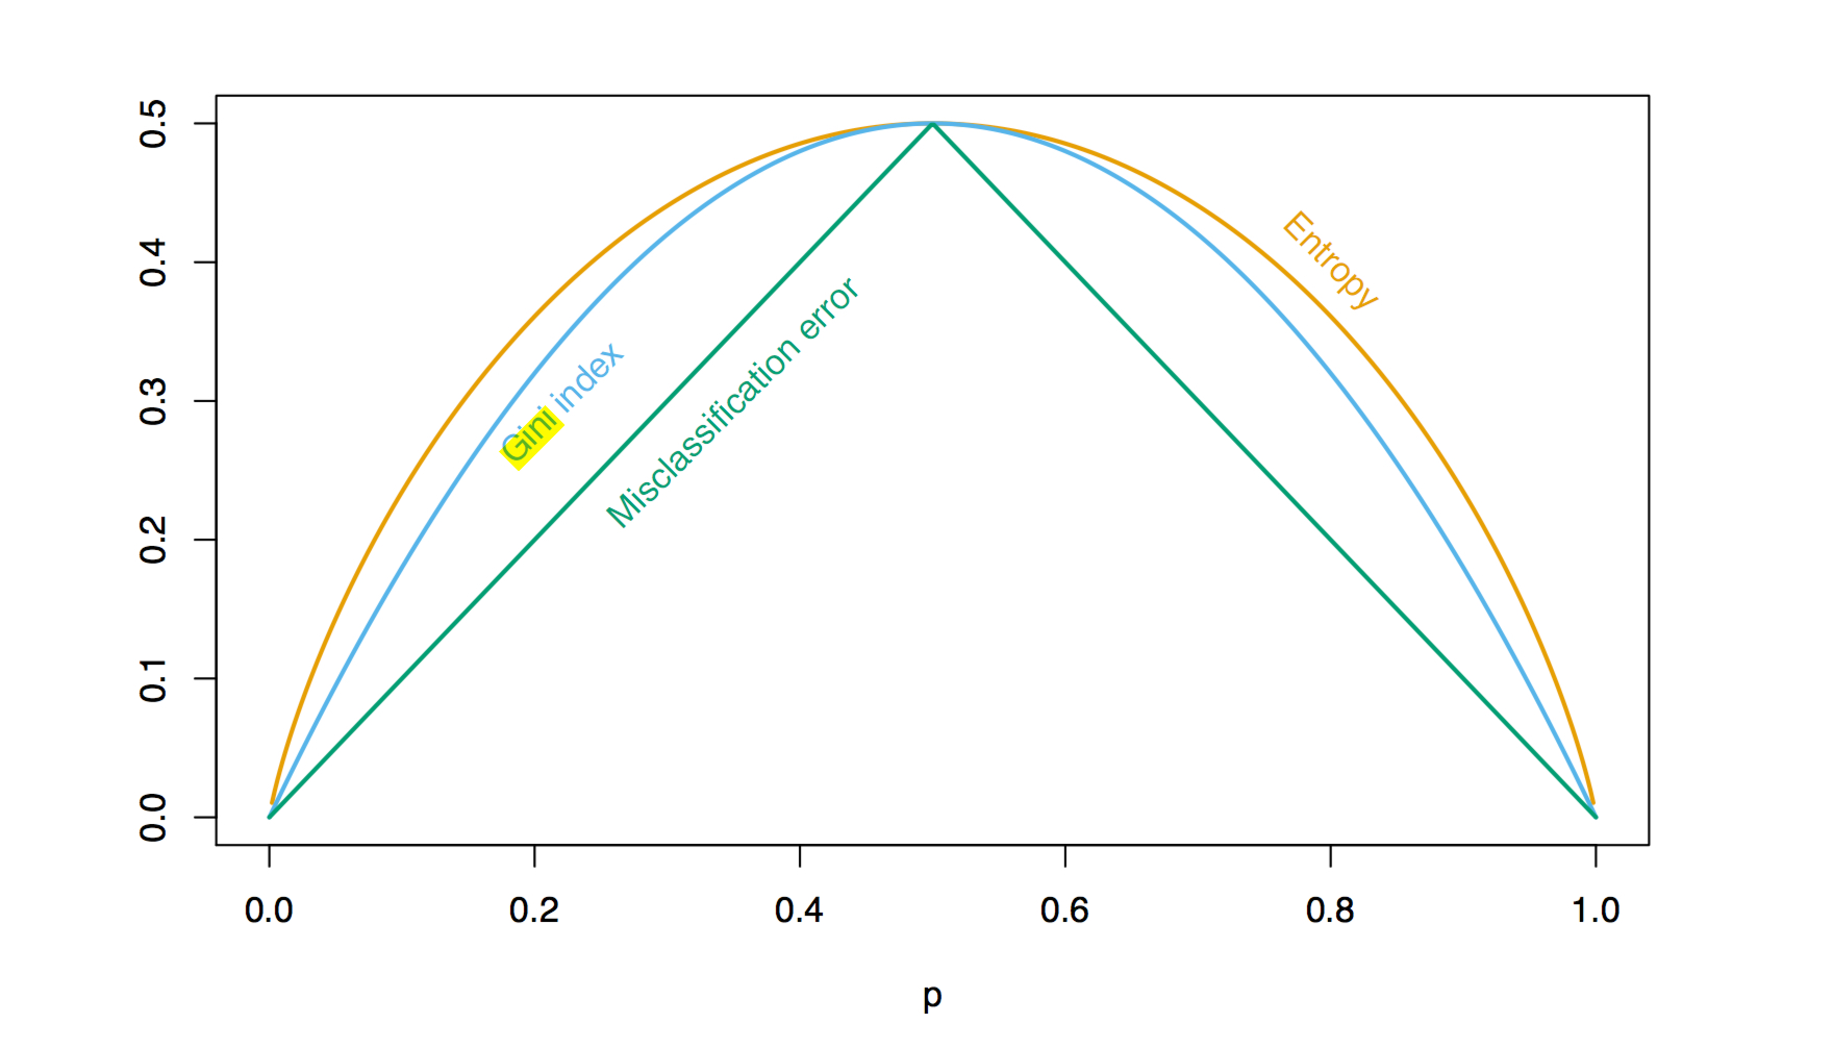
\includegraphics[width=0.8\textwidth]{ap2_figs/misclass_plot.pdf}
   \caption[Plot of misclassifcation impurity functions.]{The impurity functions vs the signal purity~\cite{esii}.}
   \label{fig:misclass_plot}
 \end{center}
\end{figure}

Additionally, the traing procedure makes use of bootstrap aggregating, known as \textit{bagging}, which performs a random re-sampling of previous events for during the tree growth.
Bagging can improve the performance in combination with the boosting procedure, which is called stochastic gradient boosting and described next.  


\subsection{Boosting}
The boosting method used in this analysis is the stochastic gradient boost, a form a gradient descent optimization for decision trees. Thus far the process begins with a single
weak classifier (a single tree). The training set will be comprised of events with {$x_{1}$,$y_{1}$}....{$x_{N}$,$y_{N}$} for N events. $x_{i}$, $y_{i} \in [0,1]$
are the input variables and class (background, signal) for event $i$. An implicit assumption in MVA training is that there exists
some function $F'(x)$, that maps a set of inputs to the event's class $y$, that is $F'(x) = y$. In training we are attempting to model this function empirically. 

The first step in gradient boosting is to grow a single tree. This single tree is $F(x)$. Surely $F(x_{i}) \neq y_{i}$ for most events, but perhaps $F(x_{i}) \approx y_{i}$
for some events. Now imagine growing a second tree $h(x)$, such that $F(x) + h(x) = y$. This second tree corrects all of the mistakes of the first, and for each event:

\begin{equation}
\begin{aligned}
\label{eqn:residual1}
%%\begin{split}
F(x_{1}) + h(x_{1}) = y_{1} \\ F(x_{2}) + h(x_{2}) = y_{2} \\ F(x_{3}) + h(x_{3}) = y_{3} \\ .... \\ F(x_{N}) + h(x_{N}) = y_{N}
%%\end{split}  
\end{aligned} 
\end{equation}

\noindent re-arranging:

\begin{equation}
\begin{aligned}
\label{eqn:residual2}
%%\begin{split}
h(x_{1}) = y_{1} - F(x_{1}) \\ h(x_{2}) = y_{2} - F(x_{2}) \\ h(x_{3}) = y_{3} - F(x_{3}) \\ .... \\ h(x_{N}) = y_{N} - F(x_{N})
%%\end{split}  
\end{aligned} 
\end{equation}

\noindent Now the second tree is grown (trained) by re-arranging the training data from the original {${$x$}_1$,$y_{1}$}....{${$x$}_N$,$y_{N}$}, to a new form:
{${$x$}_1$,$y_{1} - F(x_{1})$}....{${$x$}_N$,$y_{N} - F(x_{N})$}, where $y_{i} - F(x_{i})$ is known as the ``residuals''. Once the training of tree $h(x)$ is complete,
the model function is updated $F(x) \rightarrow F(x) + h(x)$. The role of $h(x)$ is to compensate for the shortcomings of the existing model.
This is process is repeated and trees are added to the ensemble until a specified number of trees is grown, or the improvement
from adding an additional tree is minimal. 

How is this related to gradient descent? In the gradient descent procedure, a function $J(\Theta)$, is minimized by moving in the opposite direction the gradient in steps
of finite size that are proportional to the gradient. In this way, the minimum value of $J(\Theta)$ is found for a particular $\Theta$. Starting from any value $\Theta_{i}$,
it is updated in steps according to $\Theta_{i} \rightarrow \Theta_{i} + \rho\frac{\partial~J}{\partial~\Theta_{i}}$. 
Substituing a loss function $L(F(x),y)$, in place of $J(\Theta)$, the gradient becomes $\frac{\partial L(F(x_{i}),y_{i})}{\partial F(x_{i})}$. Letting the loss function be the popular squared error loss,
$L(F(x),y) = (y-F(x))^{2}/2$, the gradient is $y_{i}-F(x_{i})$, which is the residuals found previously! Thus the negative gradient can be interpreted as the residuals for this
choice of loss function. 

\begin{equation}
\begin{aligned}
\label{eqn:residual1}
%%\begin{split}
F(x_{i}) \rightarrow F(x_{i}) + h(x_{i}) \\ F(x_{i}) \rightarrow F(x_{i}) + y_{i} - F(x_{i}) \\ F(x_{i}) \rightarrow F(x_{i}) + \frac{\partial L(F(x_{i}),y_{i})}{\partial F(x_{i})} \\ \Theta_{i} \rightarrow \Theta_{i} + \rho\frac{\partial J(\Theta_{i})}{\partial \Theta_{i}}
%%\end{split}  
\end{aligned} 
\end{equation}

\noindent where $\rho$ is the parameter that controls the step size or learning rate. It can be shown that the loss function full determines the boosting procedure. The boosting procedure
used in this analysis uses the binomial log-likelihood loss: $L(F(x),y) = ln(1+e^{-2yF(x)})$. In this loss function, the residuals are not equal to the negative gradients, which
is an advantage since the negative gradients are less sensitive to statistical outliers.

The boosting procedure begins with a single weak classifier, and produces a forest or ensemble of weak classifiers resulting in a much more performant discriminator. While the stochastic
gradient boost prodcedure is employed here, it is just one of many available boosting methods. The most popular of which includes Adaptive Boosting or AdaBoost. While AdaBoost and
gradient boosting are very similar, they differ in one significant way. As described above, gradient boosting grows additional weak classifiers with the objective being to correct
shortcomings of the existing ensemble. AdaBoost however applies weights to misclassified events in the current ensemble, therby encouring the next weak classifier to be more sensitive
to the misclassifications of the previous. Gradient boost is selected over AdaBoost due to AdaBoost's sensitivity to noisy data and outliers. 

\subsection{Pruning}
Once the ensemble of trees are completely grown after the boosting procedure, the final step known as ``pruning'' is carried out. Pruning removes leaf nodes on trees according
to a predefined critera. This process is also referred to as tree regularization. Introducing a new quantity, called risk for a single node $t$, $r(t) = p_{s}\epsilon(t)$
and the risk for the entire tree $T$, is the sum of risk over all its leaf nodes: $r(T) = \sum_{t \in L(T)} r(t)$. It is
more useful to work with the penalized risk $\widetilde{r}(T) = r(T) + \alpha|L(T)|$, where $\alpha$ is the penalty coefficient and $|L(T)|$ is the total number
of leaf nodes in tree $T$. Beginning at $\alpha = 0$, remove nodes in all trees are removed that do no lower the risk, at this first step. 
Pruning is always allowed if the penalized risk for the leaf exceeds that of its parent. At the next step, the minimum value of $\alpha$, $\alpha^{*}$ is calculated such that
the risk of the node is equal to the risk of the tree $r(t) + \alpha^{*} = r(T) + \alpha^{*}|L(T)|$. Solving for $\alpha^{*}$ provides the minimum value for $\alpha$
at the next pruning step. The optimal pruning step $m$ is acheived when $\alpha_{m} \le \alpha_{m+1}$ the optimum tree $T^{*}(\alpha_{m})$ contains $T^{*}(\alpha_{m+1})$
as a subtree. The risk is calculated on trees of an independent training subset~\cite{illya}. 


\section{Implementation}

\subsection{Hadronic Top Reconstruction BDT Training}
The hadronic top BDT is actually two BDTs with the same input variables, but trained on b-tight and b-loose events separately. The motivation for two separate trainings based on b-jet
content is the \ttbar final state in the signal region is determined by the b-jet content. A \ttbar event with two medium b-jets (b-tight) likely means that the fake lepton is either
adequately separated from the b-jet it originates from, or that the fake lepton originates from a different source entirely\footnote{It has since been shown that the performance improvement
from separate trainings is negligible compared to a single inclusive training.}. 

The number of training events used for signal and background in b-loose are 19000 and 90000 respectively.
The number of training events used for signal and background in b-loose are 13000 and 90000 respectively.
In both cases, the following hyperparameters were used in training and found to produce the best performance:

\begin{itemize}
\item Number of trees: 1000
\item Min node size: 4.5$\%$
\item Boost type: Gradient Boost
\item Shrinkage: 0.1
\item Separtion Metric: Gini index
\item Bagging fraction: 0.5
\item Number of cuts: 20
\item Maximum tree depth: 8
\end{itemize}

\noindent The number of trees is the number of weak classifiers in the ensemble or forest used in the gradient descent. The minimum node size specifies the minimum fraction of training events that must pass
through every node in each tree. Any node with fewer events is not grown. The shrinkage parameter or learning rate specifies the step size taken between each step (tree) in the gradient descent.
The bagged sample fraction is the fraction of sample events that are randomly re-sampled and used during tree growth. The number of cuts specifies the granularity over which an input variable is scanned
when selecting the best cut value. The maximum tree depth is the maximum number of nodes an event can pass through starting at the root. 

\subsubsection{b-loose}

\begin{figure}[hbtp]
 \begin{center}
   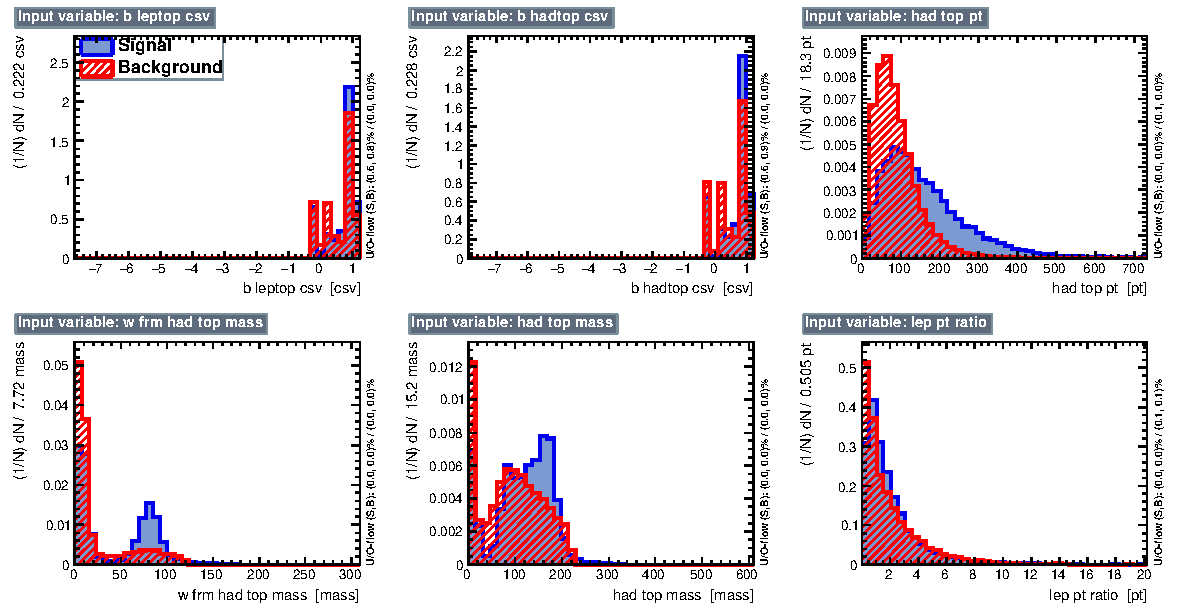
\includegraphics[width=0.8\textwidth]{ch9_figs/recoBdt_bloose/variables_id_c1.pdf}
   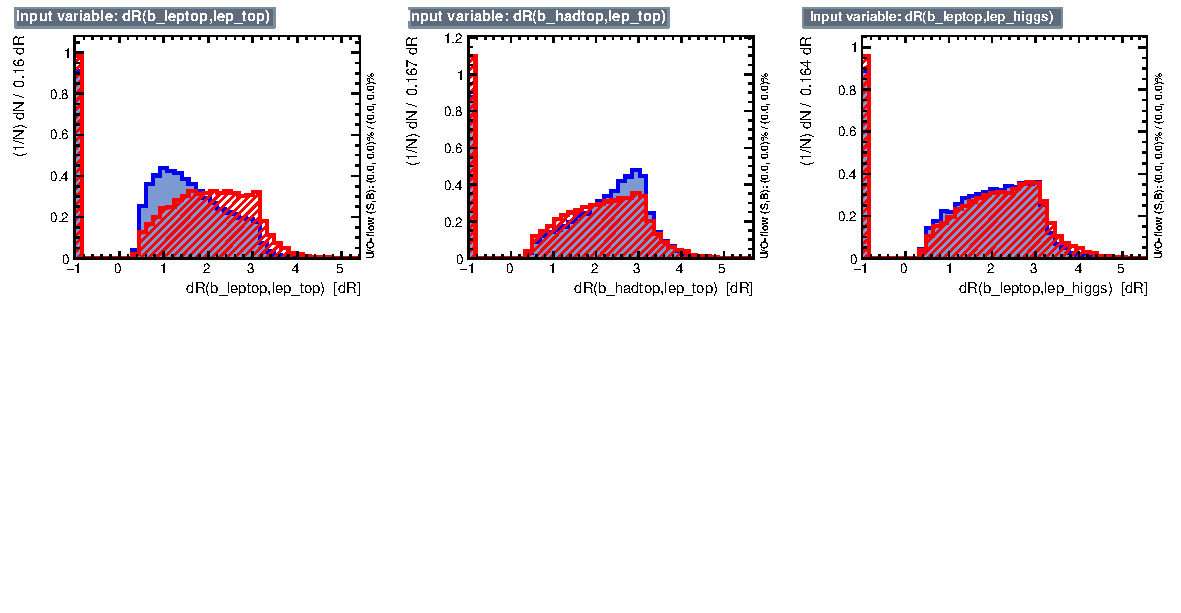
\includegraphics[width=0.8\textwidth]{ch9_figs/recoBdt_bloose/variables_id_c2.pdf}
   \caption[Input variables of the b-loose hadronic top BDT]{Input variables of the b-loose hadronic top BDT in the training samples.}
   \label{fig:recoBdt_bloose_inputs}
 \end{center}
\end{figure}

\begin{figure}[hbtp]
 \begin{center}
   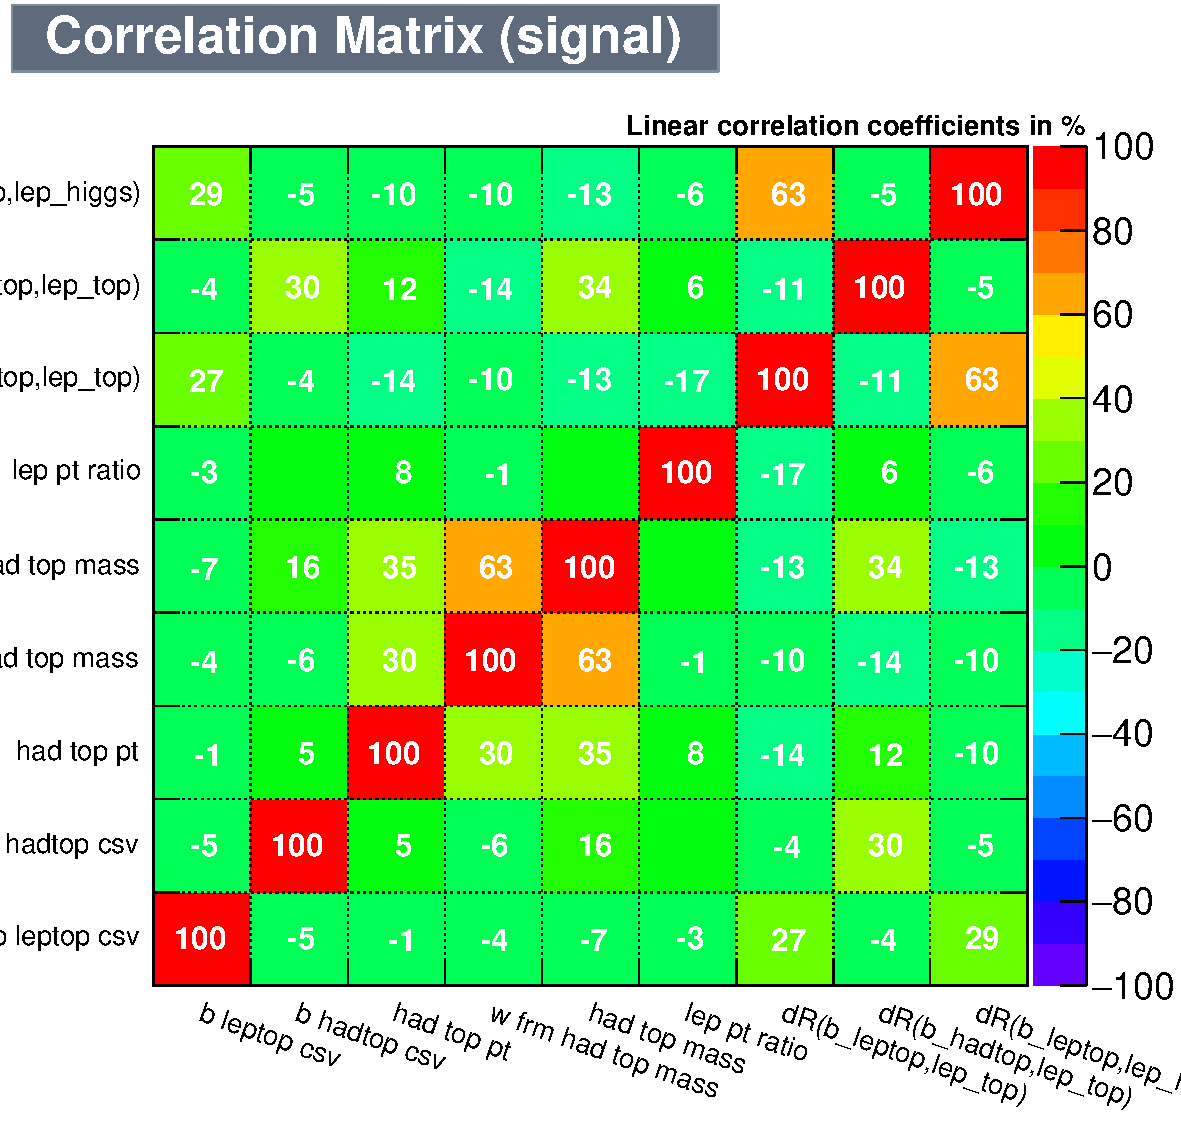
\includegraphics[width=0.49\textwidth]{ch9_figs/recoBdt_bloose/CorrelationMatrixS.pdf}
   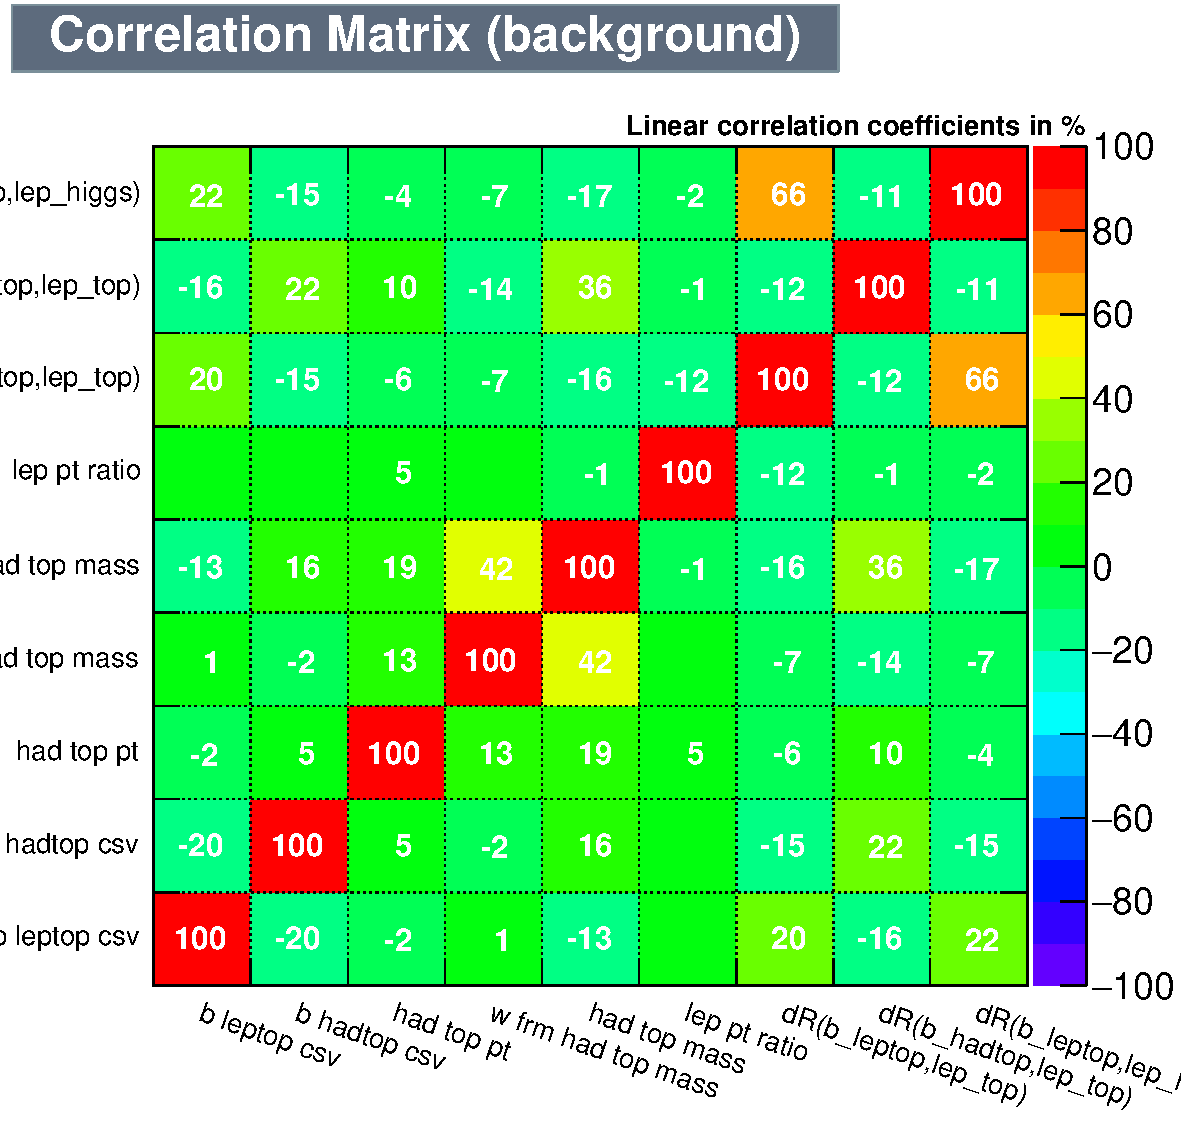
\includegraphics[width=0.49\textwidth]{ch9_figs/recoBdt_bloose/CorrelationMatrixB.pdf}
   \caption[Input variable linear correlations of the b-loose hadronic top BDT]{Input variable linear correlations in signal (left) and background (right)
     of the b-loose hadronic top BDT in the training samples.}
   \label{fig:recoBdt_b_loose_corrMatrix}
 \end{center}
\end{figure}

\begin{figure}[hbtp]
 \begin{center}
   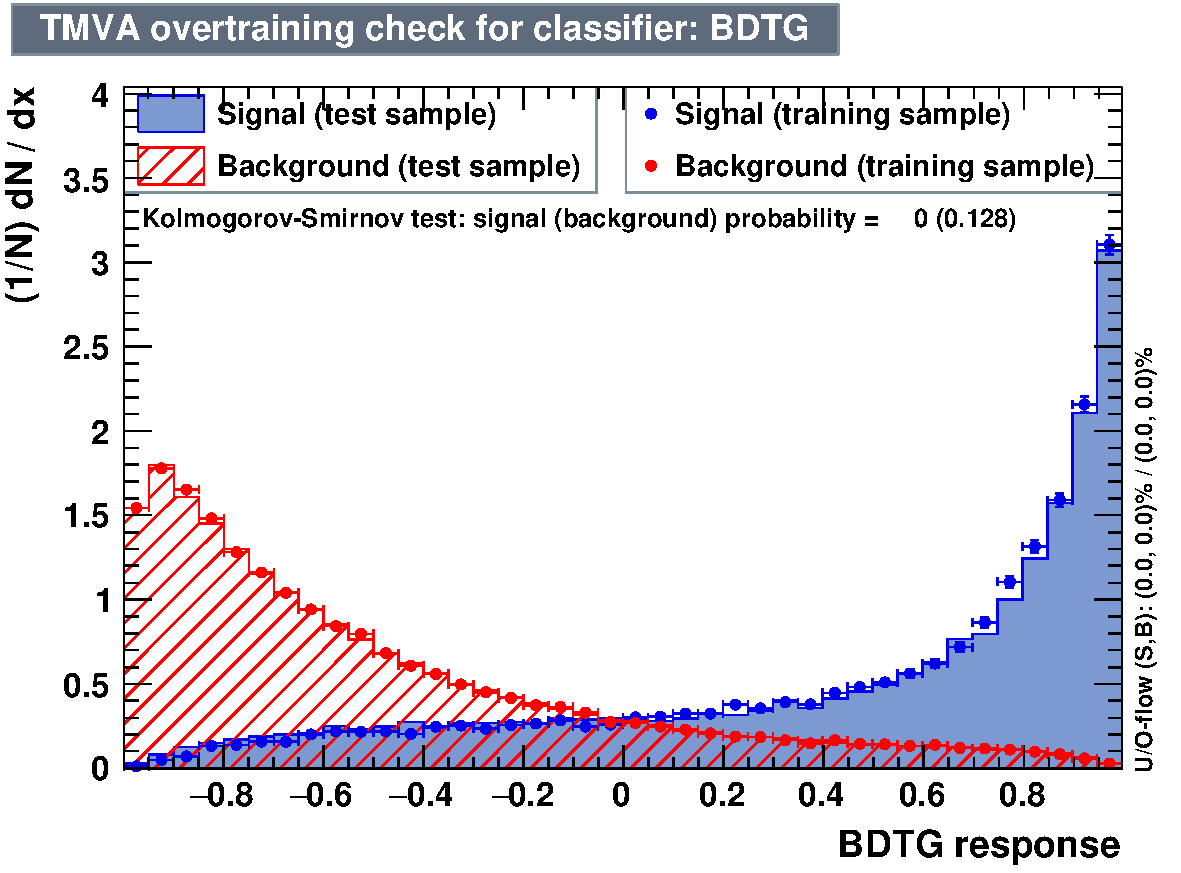
\includegraphics[width=0.8\textwidth]{ch9_figs/recoBdt_bloose/overtrain_BDTG.pdf}
   \caption[Output of the b-loose hadronic top BDT]{Output of the b-loose hadronic top BDT.}
   \label{fig:recoBdt_bloose_score}
 \end{center}
\end{figure}


\subsubsection{b-tight}

\begin{figure}[hbtp]
 \begin{center}
   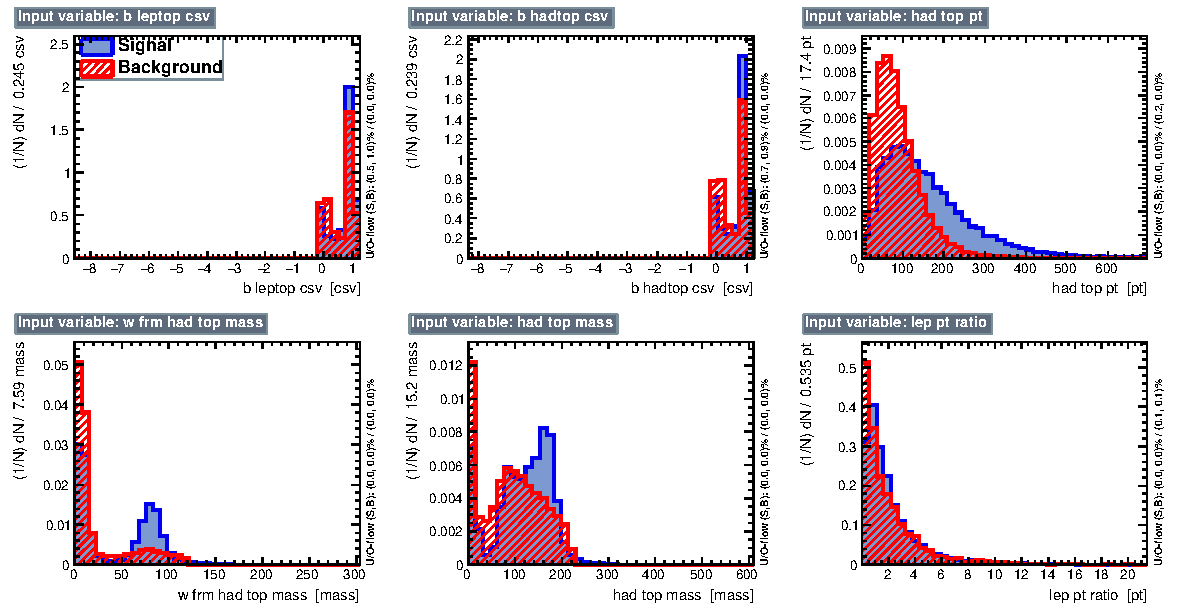
\includegraphics[width=0.8\textwidth]{ch9_figs/recoBdt_btight/variables_id_c1.pdf}
   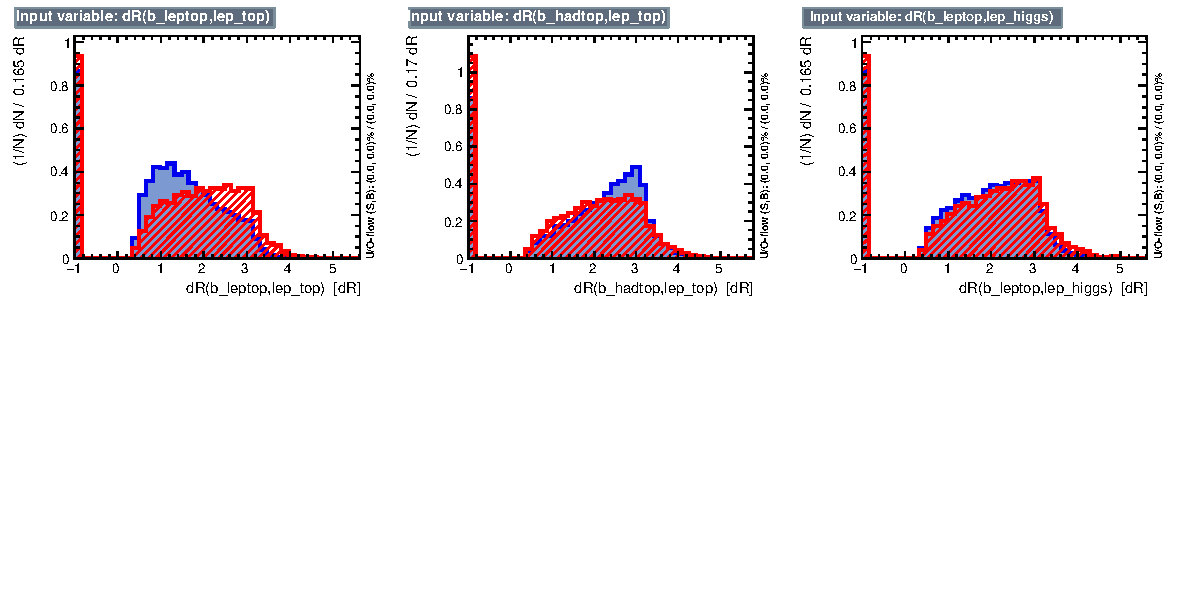
\includegraphics[width=0.8\textwidth]{ch9_figs/recoBdt_btight/variables_id_c2.pdf}
   \caption[Input variables of the b-tight hadronic top BDT]{Input variables of the b-tight hadronic top BDT in the training samples.}
   \label{fig:recoBdt_btight_inputs}
 \end{center}
\end{figure}

\begin{figure}[hbtp]
 \begin{center}
   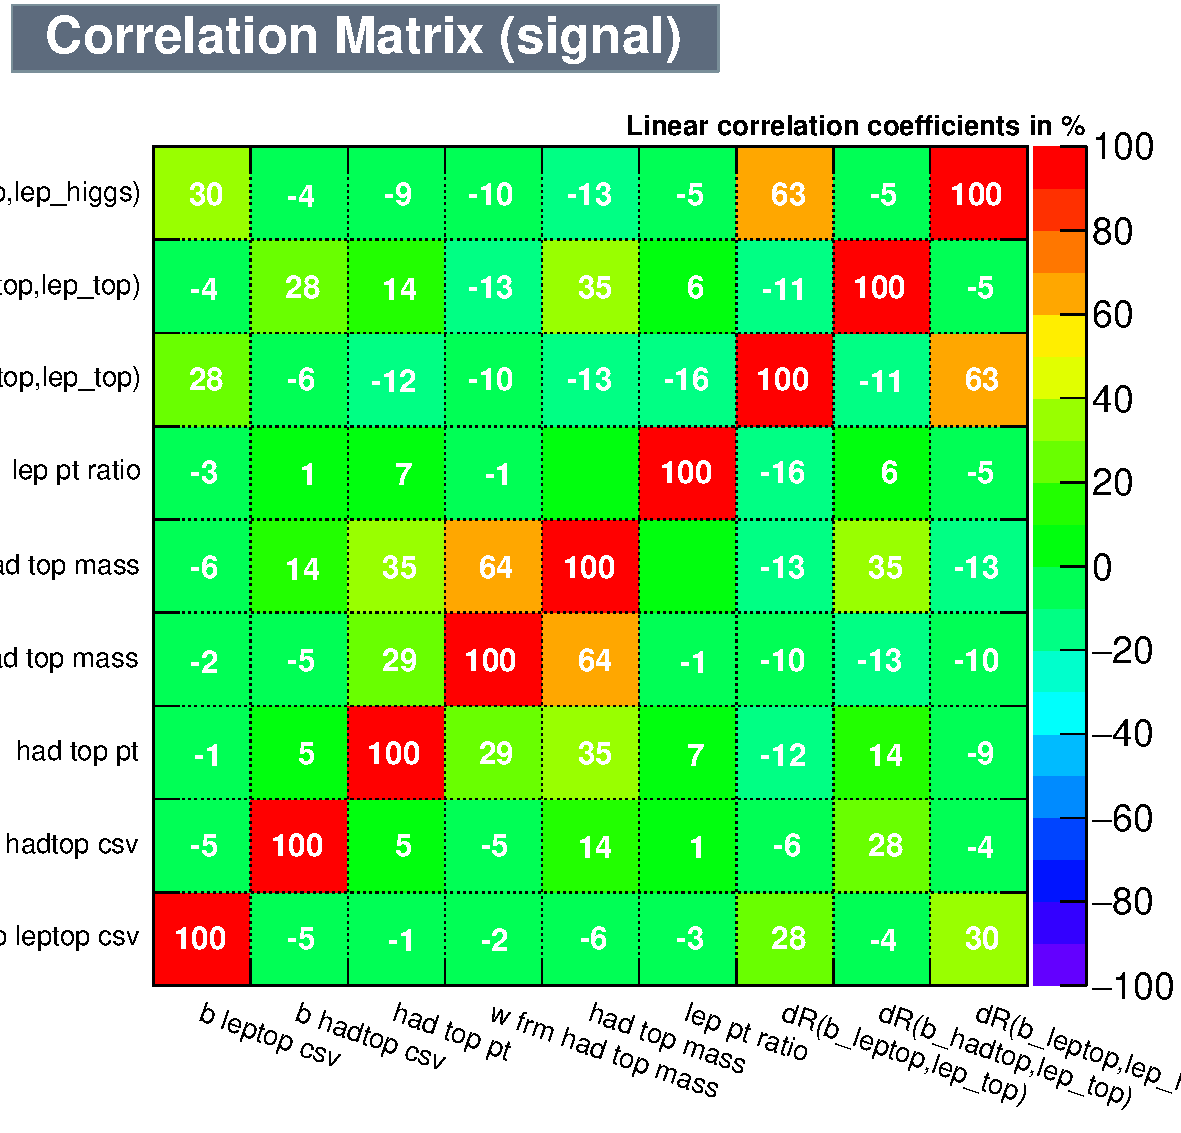
\includegraphics[width=0.49\textwidth]{ch9_figs/recoBdt_btight/CorrelationMatrixS.pdf}
   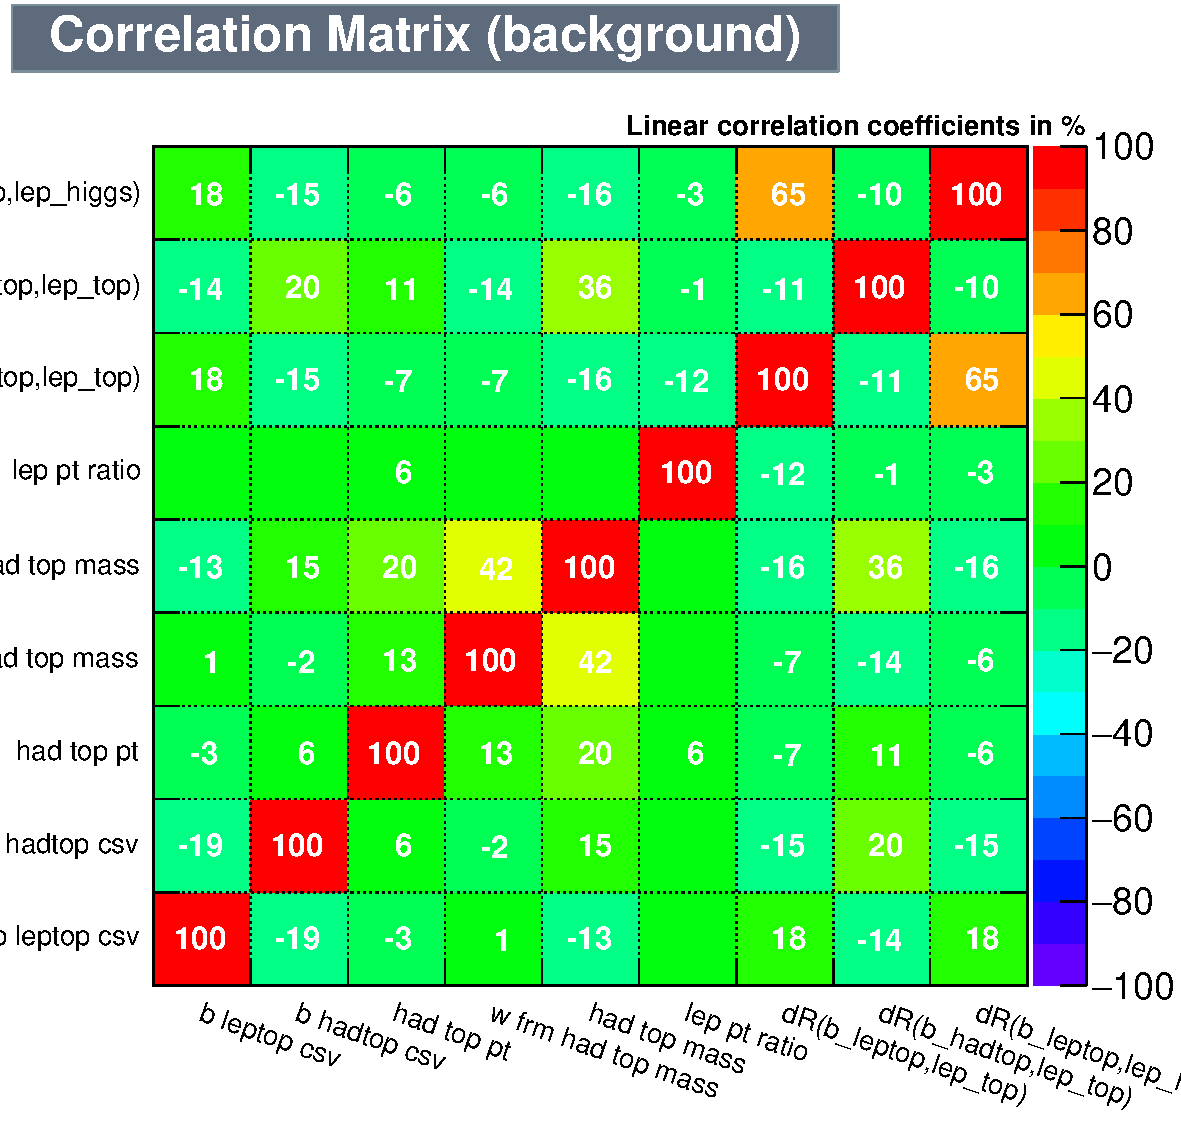
\includegraphics[width=0.49\textwidth]{ch9_figs/recoBdt_btight/CorrelationMatrixB.pdf}
   \caption[Input variable linear correlations of the b-tight hadronic top BDT]{Input variable linear correlations in signal (left) and background (right)
     of the b-tight hadronic top BDT in the training samples.}
   \label{fig:recoBdt_b_tight_corrMatrix}
 \end{center}
\end{figure}

\begin{figure}[hbtp]
 \begin{center}
   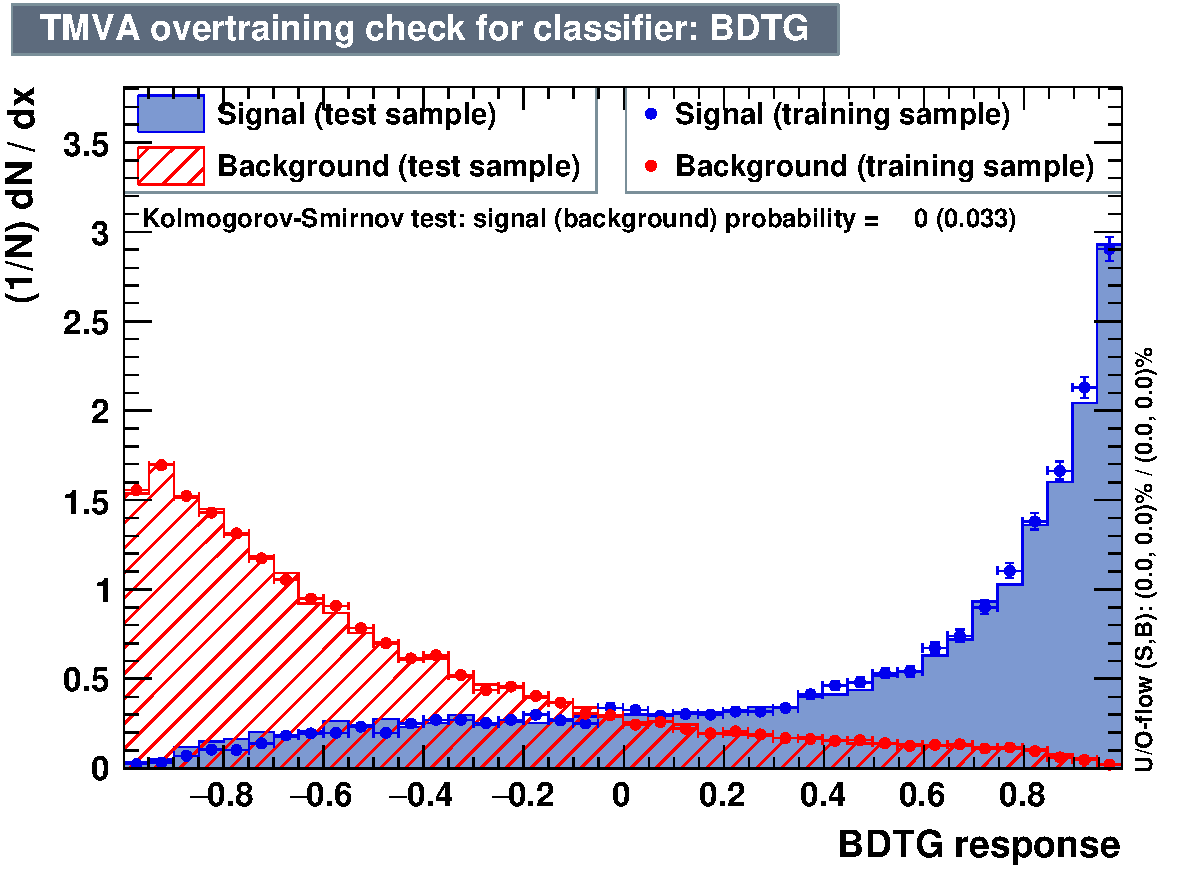
\includegraphics[width=0.8\textwidth]{ch9_figs/recoBdt_btight/overtrain_BDTG.pdf}
   \caption[Output of the b-tight hadronic top BDT]{Output of the b-tight hadronic top BDT.}
   \label{fig:recoBdt_btight_score}
 \end{center}
\end{figure}


\subsection{Final Discriminant BDT Training}

In both cases, the following hyperparameters were used in training and found to produce the best performance:
\begin{itemize}
\item Number of trees: 200
\item Minimum number of events on node: 100
\item Maximum number of nodes: 5
\item Boost type: Gradient Boost
\item Shrinkage: 0.1
\item Separtion Metric: Gini index
\item Bagging fraction: 0.6
\item Number of cuts: 200
\item Maximum tree depth: 2
\end{itemize}



\subsubsection{\ttbar}

\begin{figure}[hbtp]
 \begin{center}
   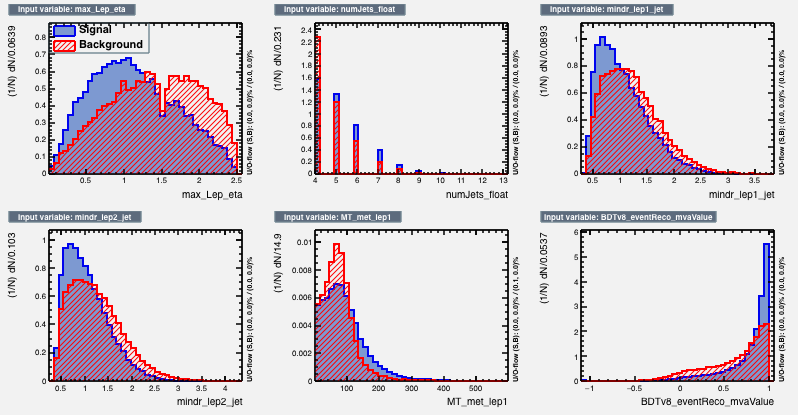
\includegraphics[width=0.8\textwidth]{ch9_figs/train_2lss_ttbar_bdtv8_value/variables_id_c1.png}
   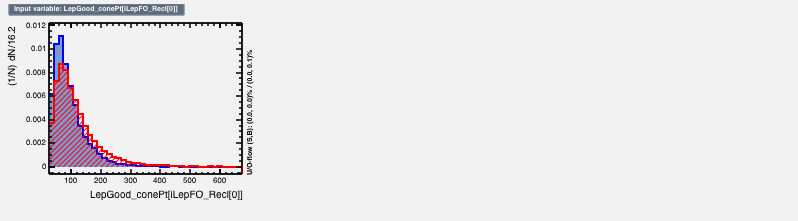
\includegraphics[width=0.8\textwidth]{ch9_figs/train_2lss_ttbar_bdtv8_value/variables_id_c2.png}
   \caption[Input variables of the BDT discriminant targeting \ttbar]{Input variables of the BDT discriminant targeting \ttbar in the training samples.}
   \label{fig:ttbarBdt_inputs}
 \end{center}
\end{figure}

\begin{figure}[hbtp]
 \begin{center}
   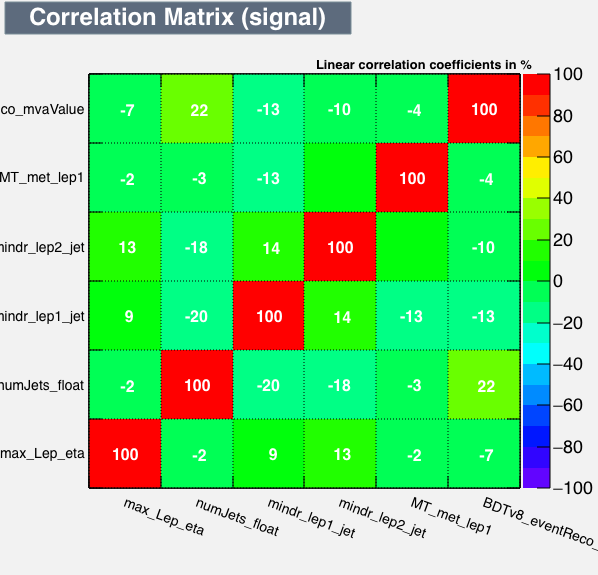
\includegraphics[width=0.49\textwidth]{ch9_figs/train_2lss_ttbar_bdtv8_value/CorrelationMatrixS.png}
   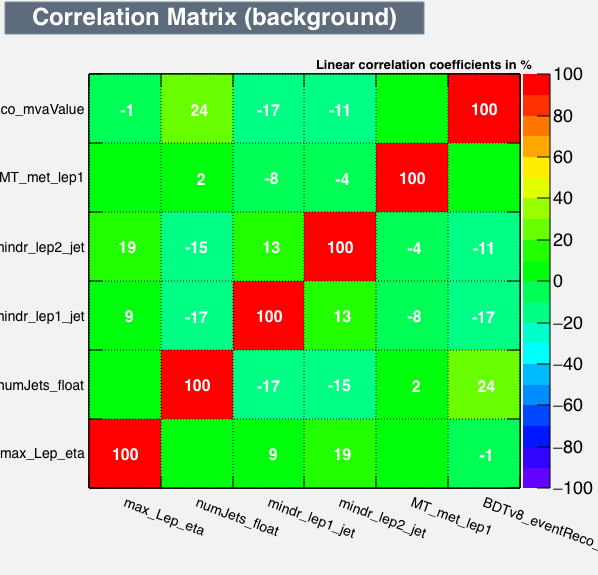
\includegraphics[width=0.49\textwidth]{ch9_figs/train_2lss_ttbar_bdtv8_value/CorrelationMatrixB.png}
   \caption[Input variable linear correlations of the BDT discriminant targeting \ttbar]{Input variable linear correlations in signal (left) and background (right)
     of the BDT discriminant targeting \ttbar in the training samples.}
   \label{fig:ttbarBdt_corrMatrix}
 \end{center}
\end{figure}

\begin{figure}[hbtp]
 \begin{center}
   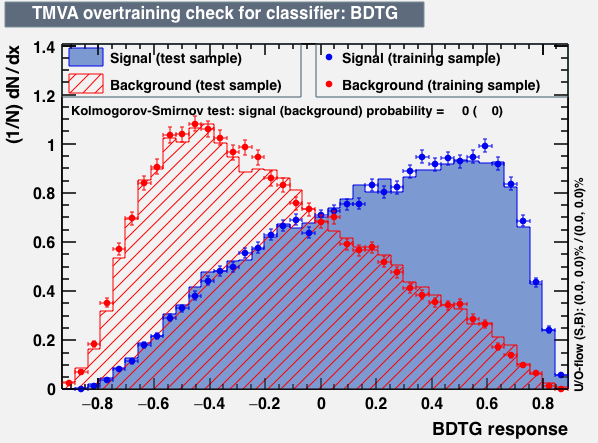
\includegraphics[width=0.8\textwidth]{ch9_figs/train_2lss_ttbar_bdtv8_value/overtrain_BDTG.png}
   \caption[Output of the BDT discriminant targeting \ttbar]{Output of the BDT discriminant targeting \ttbar in the training and testing samples.}
   \label{fig:ttbarBdt_score}
 \end{center}
\end{figure}


\subsubsection{\ttV}

\begin{figure}[hbtp]
 \begin{center}
   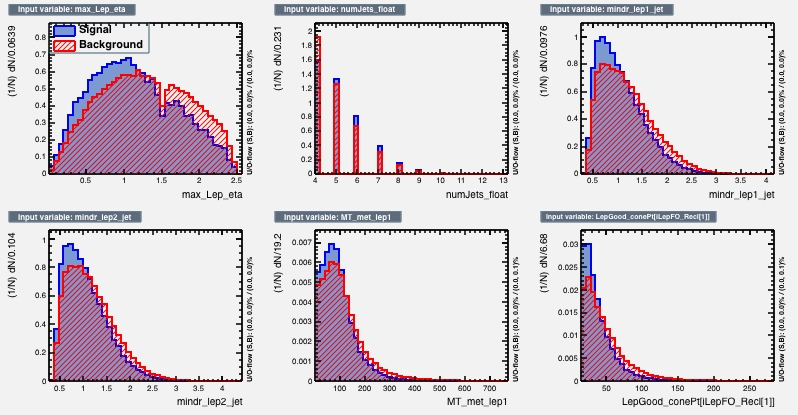
\includegraphics[width=0.8\textwidth]{ch9_figs/train_2lss_ttv_hj_value/variables_id_c1.png}
   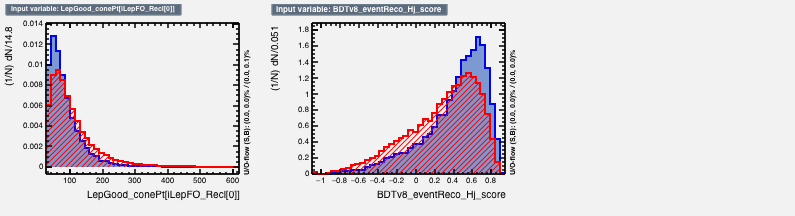
\includegraphics[width=0.8\textwidth]{ch9_figs/train_2lss_ttv_hj_value/variables_id_c2.png}
   \caption[Input variables of the BDT discriminant targeting \ttv]{Input variables of the BDT discriminant targeting \ttv in the training samples.}
   \label{fig:ttvBdt_inputs}
 \end{center}
\end{figure}

\begin{figure}[hbtp]
 \begin{center}
   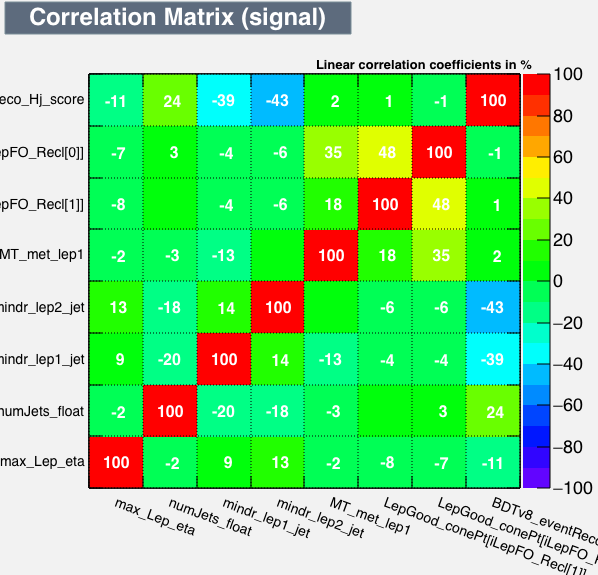
\includegraphics[width=0.49\textwidth]{ch9_figs/train_2lss_ttv_hj_value/CorrelationMatrixS.png}
   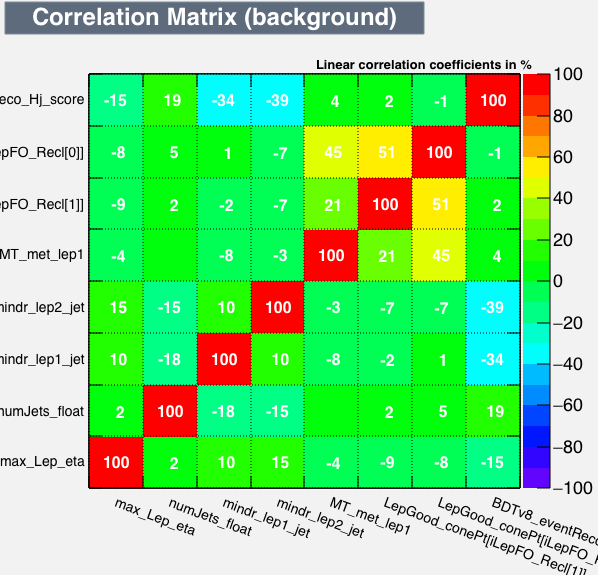
\includegraphics[width=0.49\textwidth]{ch9_figs/train_2lss_ttv_hj_value/CorrelationMatrixB.png}
   \caption[Input variable linear correlations of the BDT discriminant targeting \ttv]{Input variable linear correlations in signal (left) and background (right)
     of the BDT discriminant targeting \ttv in the training samples.}
   \label{fig:ttvBdt_corrMatrix}
 \end{center}
\end{figure}

\begin{figure}[hbtp]
 \begin{center}
   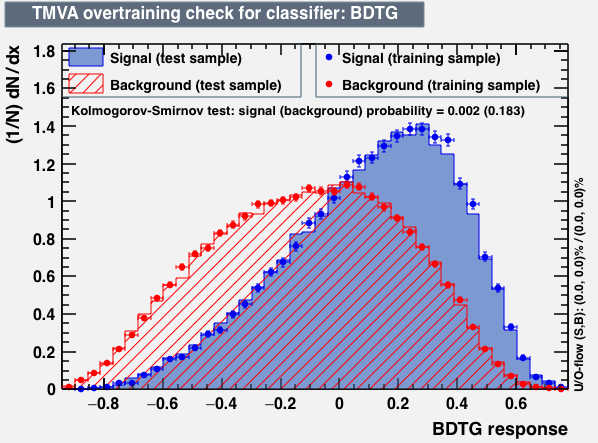
\includegraphics[width=0.8\textwidth]{ch9_figs/train_2lss_ttv_hj_value/overtrain_BDTG.png}
   \caption[Output of the BDT discriminant targeting \ttv]{Output of the BDT discriminant targeting \ttv in the training and testing samples.}
   \label{fig:ttvBdt_score}
 \end{center}
\end{figure}
